\chapter{Supersymmetry and Grand Unification: Lecture 2}

This lecture does not begin by defining supersymmetry. It does something more characteristic. It backs up. Before bosons and fermions can be related to one another, we are asked to remember what is already peculiar about fermions. Before that, we are asked to remember something peculiar about rotations themselves. The chapter should therefore be read in the same order in which the lecture unfolds: rotations, signs, exchange, loops, cancellations, broken supersymmetry, and only then the question of what an exactly supersymmetric world would look like.

The payoff is twofold. On the mathematical side, opposite signs for bosonic and fermionic loops create the possibility of cancellation. On the physical side, exact supersymmetry would radically alter ordinary matter. Between those two observations lies the lecture's real theme: supersymmetry is interesting precisely because exact supersymmetry is not the world we live in.

\section{Rotations, \(2\pi\), and the Topological Prehistory of Supersymmetry}

``Actually before we talk about supersymmetry,'' Susskind says, ``we should talk again about fermions and bosons.'' Then he backs up once more: before fermions, rotations in space. The familiar statement that a rotation by \(2\pi\) is the same as no rotation at all is, in the topological sense relevant here, too naive. He demonstrates the point physically with his arm, and then translates it into the box-and-ball picture.

We imagine a ball in a box, connected to the walls by strings. The walls represent spatial infinity, so the box is held fixed. A rotation of the ball by \(2\pi\) tangles the strings, and the tangle cannot be removed if the ball is not rotated further. A rotation by \(4\pi\), however, can be undone by moving the strings around the ball. He jokingly says he has already proved the theorem ``by hand-waving.'' That is enough for the lecture. The point is not a formal homotopy proof; the point is the qualitative fact that \(2\pi\) is not topologically trivial, while \(4\pi\) is.

This is the geometric memory that later reappears in fermions. In one of the discussion remarks Susskind even says, roughly, that bosons behave as though there were no strings attached to the wall, whereas fermions remember that a \(2\pi\) rotation has taken place.

Now we freeze the position of a particle and look only at its spin state. Following the lecture, we may temporarily call that state \(\ket{S}\); more generally we write \(\ket{\psi}\). The simplest possibility is that a \(2\pi\) rotation acts by multiplication with a number:
\begin{equation}
R(2\pi)\ket{\psi}=\xi\ket{\psi}.
\end{equation}
If we perform the same rotation twice, then
\begin{equation}
R(4\pi)\ket{\psi}=\xi^2\ket{\psi}.
\end{equation}
But the topological statement was precisely that \(4\pi\) is equivalent to doing nothing. Therefore
\begin{equation}
R(4\pi)\ket{\psi}=\ket{\psi},
\qquad
\xi^2=1,
\qquad
\xi=\pm 1.
\end{equation}
So the state may come back to itself after a \(2\pi\) rotation either with a plus sign or with a minus sign:
\begin{equation}
R(2\pi)\ket{\psi_{\mathrm{boson}}}=+\ket{\psi_{\mathrm{boson}}},
\qquad
R(2\pi)\ket{\psi_{\mathrm{fermion}}}=-\ket{\psi_{\mathrm{fermion}}}.
\end{equation}

That already separates bosons from fermions in a very stark way. The lecture emphasizes that such a rotation is not merely formal. One can implement it in the laboratory by letting a spin precess in a magnetic field, or by rotating the magnetic field itself. The mathematical distinction is therefore physically meaningful, if only we can find the right way to see it.

\section{Spin States Under Rotation and the Interference Test of a Sign Change}

At first sight a minus sign seems like no physics at all. If we rotate every copy of a wavefunction by \(2\pi\) and the result is just \(-\Psi\), then every observable constructed from \(\Psi^*\Psi\) is unchanged. That is exactly the paradox the lecture wants to raise before it resolves it.

\subsection{Question \& Answer}

Can the minus sign from a \(2\pi\) rotation ever be observed?

Yes, but only as a relative sign.

The lecture answers with a two-path interference experiment. A single electron is prepared in a superposition of two branches, one going through an upper path and one through a lower path. If the two branches are \(\psi_1\) and \(\psi_2\), then before anything is rotated the total wavefunction is
\begin{equation}
\Psi=\psi_1+\psi_2.
\end{equation}
Now imagine that while the electron is trapped in one of the two regions, we rotate only one branch by \(2\pi\). For a fermion, that branch picks up a minus sign. If it is the second branch that is rotated, the recombined state becomes
\begin{equation}
\Psi'=\psi_1-\psi_2.
\end{equation}
So the physical question is not whether \(\Psi\) differs from \(-\Psi\). The physical question is whether
\begin{equation}
\psi_1+\psi_2
\qquad \text{or} \qquad
\psi_1-\psi_2
\end{equation}
emerges after recombination.

If the two returning wave packets are symmetric by reflection about the center of the screen, then the odd combination must vanish there:
\begin{equation}
\Psi_{\mathrm{odd}}(0)=0.
\end{equation}
That is the cleanest way to state the lecture's argument. A relative minus sign shifts the interference pattern; maxima become minima, and the electron is never found at the symmetry point. On the other hand, if both branches are rotated together, the full state changes only by an overall sign, and then nothing observable happens:
\begin{equation}
|\Psi|^2 = (-\Psi)^*(-\Psi).
\end{equation}

This is why the sign under \(2\pi\) is real physics but only in a relational way. Rotating half the experiment relative to the other half is like rotating the ball relative to the box: memory can then be detected. Rotating the whole experiment together is like rotating ball and box together: the effect disappears. And if the relative rotation were \(4\pi\), the extra sign would disappear as well.

The lecture also makes a useful contrast here. The special role of \(2\pi\) is that it changes only the sign of a fermion state while leaving the spin orientation effectively the same. A generic rotation changes the spin state more substantially. Then the two branches are no longer the same object up to a sign, and the interference pattern is partially washed out or even destroyed. A \(180^\circ\) flip, for example, destroys it completely.

\section{Bosons, Fermions, and Exchange Symmetry}

Having extracted one distinction between bosons and fermions from rotations, the lecture turns to a second one: exchange symmetry. This shift is not accidental. The next target is a sign rule for Feynman loops, and that rule depends on what happens when identical particles are interchanged.

Let \(\Psi(1,2)\) be the two-particle wavefunction, and let \(P_{12}\) denote the operator that exchanges particles \(1\) and \(2\). Then the standard statements are
\begin{align}
P_{12}\Psi(1,2)&=+\Psi(1,2), \qquad \Psi(1,2)=+\Psi(2,1)
\qquad \text{for bosons},\\
P_{12}\Psi(1,2)&=-\Psi(1,2), \qquad \Psi(1,2)=-\Psi(2,1)
\qquad \text{for fermions}.
\end{align}
The lecture phrases this more directly: bosonic wavefunctions are symmetric, fermionic wavefunctions are anti-symmetric.

The board evidence is especially useful here because Susskind is speaking in ket language at this moment, not only in coordinate language.

\begin{figure}
\centering

\includegraphics[width=0.74\textwidth]{lecture_02_figure_02.png}
\caption{Fermion anti-symmetry and state-label sketch. The screenshot is kept because it preserves the board layout and the ket-style presentation, even though only \(\ket{S}\) is securely legible.}
\end{figure}

The only symbol that is really clear on the board is \(\ket{S}\). So the cleaned equations have to be treated as careful reconstructions rather than verbatim board transcriptions. The mathematically appropriate statements are
\begin{align}
\Psi(1,2)&=-\Psi(2,1),\\
P_{12}\ket{\psi}&=-\ket{\psi}.
\end{align}
The second line is the lecture's ket-language version of the same fact. It is this minus sign under exchange, not some abstract slogan about statistics, that is about to reappear in the sign of a closed fermion loop.

\section{Why a Closed Fermion Loop Carries a Minus Sign}

We now come to what Susskind calls ``yet another question'': a question about very simple Feynman diagrams. These are vacuum diagrams with no external lines, just a closed loop in empty space. One may think of the loop either as a particle moving around a closed curve in spacetime or, more physically, as pair creation followed by annihilation. The precise integral associated with the diagram is not the point here. The point is the sign.

\subsection{Question \& Answer}

Why does one closed fermion loop come with a minus sign?

The lecture gives an elegant proof that uses nothing heavier than exchange symmetry.

Begin with two disconnected loops. Since disconnected diagrams multiply, the sign of the two-loop diagram is the square of the sign of the one-loop diagram:
\begin{equation}
\operatorname{sign}(\text{two disconnected loops})
=
\bigl(\operatorname{sign}(\text{one loop})\bigr)^2
=
+1.
\end{equation}
So two disconnected loops always carry an overall plus sign, regardless of whether one loop by itself is positive or negative.

Now cut both loops at a common time slice. At that instant we see two identical particles. There are then two possibilities: reconnect them without exchanging the particles, or interchange the two particles before reconnecting them. The first operation gives back the original two disconnected loops. The second changes the amplitude by the exchange sign:
\begin{enumerate}
\item For bosons, exchanging the two particles contributes no extra sign.
\item For fermions, exchanging the two particles contributes a minus sign.
\end{enumerate}
But after this interchange and reconnection, what had been two loops has become one single loop. Therefore the sign of the one-loop diagram must be
\begin{equation}
\operatorname{sign}(\text{one closed boson loop})=+1,
\qquad
\operatorname{sign}(\text{one closed fermion loop})=-1.
\end{equation}

That is the whole proof. It is not a path-integral derivation, and the lecture does not want one here. It wants the elementary mechanism to be visible: the extra minus sign comes from exchanging identical fermions. The consequences are immediate. Bosonic and fermionic loops contribute with opposite signs to quantum corrections. We have finally reached the first real mathematical doorway into supersymmetry.

\section{Vacuum Energy, Boson Self-Energy, and the Zeroth-Order Supersymmetry Idea}

The first place Susskind uses the loop-sign result is the vacuum energy. A closed boson loop contributes with one sign; a closed fermion loop contributes with the opposite sign. Since the observed vacuum energy is astonishingly small compared with the naive quantum field theoretic estimate, the lecture pauses over the fact that cancellation is at least possible.

All things being equal, meaning the same mass and the same relevant quantum numbers, a boson and a fermion would give equal contributions in magnitude and opposite contributions in sign. Schematically,
\begin{equation}
m_{\text{partner}}=m_{\text{particle}},
\qquad
Q_{\text{partner}}=Q_{\text{particle}},
\end{equation}
and then one may hope for
\begin{equation}
\Delta E_{\mathrm{vac}}^{(b)}+\Delta E_{\mathrm{vac}}^{(f)}=0.
\end{equation}
The lecture is careful not to oversell this. It does not say that the cosmological constant problem has been solved. It says only that the sign structure creates room for cancellation, which is already something important.

Then comes one of Susskind's characteristic pivots: ``another thought to keep in mind.'' Vacuum energy is not the main issue. The sharper question is whether the same logic can help with the self-energy of bosons, especially Higgs-like scalars. Bosonic loop corrections by themselves drive scalar masses upward. Fermions, by contrast, can be protected against such enormous corrections. So if a theory forced bosons and fermions to travel in closely matched pairs, one could imagine transferring that protection to the bosons. In schematic form,
\begin{equation}
\Delta m_B^2\big|_{\text{boson loop}}
+
\Delta m_B^2\big|_{\text{fermion loop}}
\approx 0.
\end{equation}
Exact partner matching would give exact cancellation. Near matching would give only approximate cancellation, but approximate cancellation is enough if the goal is merely to keep the Higgs sector from running away to enormous scales.

After the break, the lecture rephrases the whole idea ``to zeroth order,'' not in the strict mathematical sense of an expansion, but as a rough first picture. The rough picture is that every particle in nature comes with a superpartner of the opposite statistics. Here ``statistics'' is exactly Susskind's word for fermion-ness versus boson-ness. Supersymmetry, at this stage of the lecture, is the hypothesis that the spectrum is doubled in just this way.

The board at this point is valuable mainly as layout evidence: simple loops on the left, more elaborate loop-corrected structures on the right.

\begin{figure}
\centering

\includegraphics[width=0.8\textwidth]{lecture_02_figure_04.png}

\begin{tikzpicture}[scale=0.95]
\draw (-4.8,0) circle (0.65);
\draw (-2.4,0) circle (0.65);
\draw (0.4,0) -- (3.8,0);
\fill (2.1,0) circle (0.06);
\draw (2.1,0) -- (2.1,0.28);
\draw (2.1,0.95) circle (0.67);
\end{tikzpicture}

\caption{Loop-diagram comparison in the supersymmetry discussion. The redraw is intentionally schematic: the left-hand side shows simple loop topologies, while the right-hand side suggests loop corrections to propagating particles.}
\end{figure}

The lecture still has not defined the supersymmetry algebra. It is doing something more primitive and, pedagogically, more effective. It is giving us a reason to want such a symmetry in the first place.

\section{Broken Supersymmetry, Naturalness, and Experimental Reach}

At this point the lecture turns from motivation to reality. Exact mass matching would give exact cancellation, but exact mass matching is not how nature looks. We know this at once from experiment. If there were a bosonic partner of the electron with the same charge and the same mass, it would already have shown up in ordinary production processes. An electron-positron pair can annihilate into a virtual photon, and if the partner were truly degenerate with the electron, the virtual photon could produce the partner pair just as easily:
\begin{equation}
e^-e^+ \to \gamma^\ast \to \tilde e^- \tilde e^+.
\end{equation}
We do not see that. So exact supersymmetry is not the world we live in.

\subsection{Question \& Answer}

If supersymmetry helps, why have we not seen the partners?

Because the symmetry, if it exists in nature, must be broken.

The lecture insists on two points at once. First, the masses of particles and superpartners are certainly not equal. Second, the splittings cannot be arbitrarily large if supersymmetry is supposed to do the job for which it was invented. Exact degeneracy would produce exact cancellation. Near degeneracy gives approximate cancellation. But if the partner masses were pushed all the way up to some enormous scale, then the cancellations would be poor and the Higgs self-energy problem would simply return in a slightly disguised form.

This is the naturalness argument in the form the lecture wants it. If superpartners were as heavy as the unification scale or the Planck scale, their loops would drag the Higgs sector upward almost as badly as if there were no supersymmetry at all. So a supersymmetry that protects the Higgs mass requires that the particle-superpartner splittings not be too large. Susskind gives a lecture-era estimate of order a few hundred GeV as the scale beyond which the cancellation becomes too poor to be convincing. The exact number should be taken historically rather than timelessly; the logical point is the important one.

The lecture also rejects a merely aggregate cancellation, where the sum of all fermionic effects accidentally cancels the sum of all bosonic effects. That would be just another fine-tuning. The supersymmetric hope is a structured cancellation, enforced by a symmetry, not a miraculous bookkeeping accident.

Here the line-style contrast between ordinary loops and partner loops becomes visually explicit.

\begin{figure}
\centering

\includegraphics[width=0.78\textwidth]{lecture_02_figure_05.png}

\begin{tikzpicture}[scale=0.95]
\draw (-2.1,0) circle (1.0);
\draw[dashed] (2.1,0) circle (1.0);
\end{tikzpicture}

\caption{Solid and dashed loop topologies. The essential content is the side-by-side comparison of ordinary and superpartner loop contributions with different statistics and therefore opposite signs.}
\end{figure}

The lecture then sharpens the matching requirement. It is not enough that masses be comparable. Couplings must match as well. Once external photons are attached to the loop, cancellation requires that the partner carry the same electric charge as the original particle:
\begin{equation}
Q_{\text{partner}}=Q_{\text{particle}}.
\end{equation}
Otherwise the two diagrams do not have the same numerical coefficient and the cancellation fails.

Experimentally, there are then two fronts. One may look directly for superpartner production in sufficiently energetic collisions. Or one may look indirectly for their virtual effects in high-precision electroweak processes. The lecture emphasizes that electron-positron machines are cleaner for the second purpose than hadron colliders, because protons are composite and the collision environment is correspondingly messy. The high-precision data do constrain supersymmetry, but in the lecture's discussion they do not yet rule it out.

Susskind also remarks that most superpartners would not be expected to sit around forever. They should decay, perhaps cascading down to a lightest superpartner. In many models that lightest state is neutral and may be stable. But the main phenomenological message of the lecture is simpler: if supersymmetry is to protect the Higgs sector, the new particles must lie not too far beyond experimental reach.

\section{Exact Supersymmetry Would Destroy Ordinary Chemistry}

Before closing, the lecture fixes the relation between the spins of particles and their superpartners. Bosons are paired with fermions, fermions with bosons, and the spin changes by half a unit:
\begin{equation}
j_{\text{superpartner}}=j\pm\frac{1}{2}.
\end{equation}
Thus a gauge boson has a spin-\(\tfrac12\) partner, while an ordinary spin-\(\tfrac12\) fermion such as the electron has a scalar partner. This is also where the familiar names appear. Bosonic particles acquire fermionic partners with ``-ino'' names such as photino and Higgsino, whereas fermions acquire bosonic partners such as the selectron and the squark. The lecture also notes that extra scalar fields raise the danger of additional spontaneous symmetry breaking, which would generally be unwelcome and must be controlled.

There is a brief aside about lower dimensions: in two spatial dimensions the boson-fermion dichotomy is generalized, and one finds anyons with more general spin-statistics behavior. The lecture does not pursue that topic further. Instead it asks the question with which it really wants to end.

\subsection{Question \& Answer}

What would the world be like if supersymmetry were exact?

Very different. In particular, ordinary chemistry would fail.

Here ``exact'' means exact degeneracy between particles and superpartners. If that were true, the electron would have a bosonic partner with exactly the same mass and charge, and the photon would have a massless fermionic partner, the photino:
\begin{equation}
m_\gamma=0
\qquad \Rightarrow \qquad
m_{\tilde\gamma}=0.
\end{equation}
Now consider an atom with more than two electrons. In hydrogen and helium the available electrons occupy the lowest orbit. In lithium and heavier atoms, outer electrons sit farther out because the low-lying states are blocked by the Pauli exclusion principle. The outer electron wants to fall inward, but ordinary Fermi statistics forbids it.

In an exactly supersymmetric world there is a new escape route. The outer electron can emit a photino and turn into a selectron:
\begin{equation}
e^-_{\text{outer}} \to \tilde e^- + \tilde\gamma.
\end{equation}
That is the key move in the lecture's final argument. The emitted particle is a fermion, so what remains must be a boson. Once the electron has turned into a selectron, Pauli blocking no longer applies. The selectron can drop to the lowest orbit.

\begin{figure}
\centering

\includegraphics[width=0.72\textwidth]{lecture_02_figure_06.png}

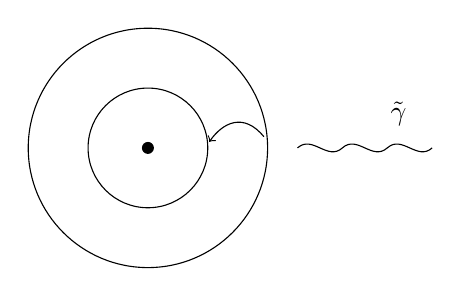
\begin{tikzpicture}[scale=0.95]
\fill (0,0) circle (0.08);
\draw (0,0) circle (0.8);
\draw (0,0) circle (1.6);
\draw[->] (1.55,0.15) .. controls (1.28,0.48) and (1.0,0.34) .. (0.82,0.08);
\draw (2.0,0) .. controls (2.2,0.18) and (2.4,-0.18) .. (2.6,0)
            .. controls (2.8,0.18) and (3.0,-0.18) .. (3.2,0)
            .. controls (3.4,0.18) and (3.6,-0.18) .. (3.8,0);
\node at (3.35,0.45) {$\tilde\gamma$};
\end{tikzpicture}

\caption{Radiative drop to a lower orbit. The board shows emitted radiation and an inward transition; the photino label in the redraw is supplied from the transcript rather than from a legible board inscription.}
\end{figure}

The force of the argument is cumulative. It is not only one outer electron in a lithium-like atom that would do this. Valence electrons more generally would have the same route available to them. They would convert into bosonic selectrons and fall inward. Instead of ordinary shell structure, one would have something closer to a Bose condensate of selectrons gathered near the nucleus. Whatever such a world might be, it would not support familiar atoms, familiar valence structure, or familiar chemistry.

The lecture even anticipates the obvious objection: perhaps the coupling for this transition is tiny. But here there is no escape of that sort. The relevant coupling is electromagnetic. In the lecture's rough estimate, a lithium-like atom would not linger in its ordinary form for long at all; the transition would be rapid on atomic timescales.

So the closing lesson is not merely that exact supersymmetry is experimentally excluded. It is that exact supersymmetry would make a world unlike ours. Susskind's answer to the question ``why is the symmetry broken?'' is correspondingly blunt: if it were not broken, we would not be here to ask. That is not a complete theory of supersymmetry breaking, but it is the right final physical punch.

\section{Summary}

The lecture reaches supersymmetry by refusing to define it too early. First we learn that a \(2\pi\) rotation is not topologically as innocent as it seems, whereas a \(4\pi\) rotation is. Then we learn that a spin state may therefore come back under \(2\pi\) with a sign, and that fermions pick up \(-1\) while bosons do not. Then the sign is made observable through interference, where relative minus signs shift the pattern even though global ones do not.

Only after that does the lecture turn to exchange symmetry and then to Feynman loops. Anti-symmetry under exchange implies that a single closed fermion loop comes with a minus sign, whereas a boson loop comes with a plus sign. From there the supersymmetric idea becomes natural: if bosons and fermions occur in sufficiently matched pairs, their quantum corrections can cancel. That possibility first appears in the vacuum energy and then, more importantly for the lecture, in the self-energy of bosons.

Nature, however, does not realize the exact version of the idea. The partners are not degenerate with the known particles, so supersymmetry, if it exists, must be broken. But it cannot be broken too badly if it is to protect the Higgs sector from enormous radiative corrections. And if it were not broken at all, ordinary chemistry would collapse. That is the balance the lecture leaves us with: supersymmetry is interesting because it can cancel dangerous quantum effects, and it must be broken because an exactly supersymmetric world would not look anything like ours.